Analisis masalah pada Subbab~\ref{sec:03-analisis-masalah}, serta analisis sistem serupa pada Subbab~\ref{sec:03-analisis-sistem-serupa}, menghasilkan gambaran mengenai fitur dan karakteristik yang harus dimiliki oleh sistem. Dari sini disusun kebutuhan fungsional yang menjelaskan layanan apa saja yang harus disediakan oleh sistem, serta kebutuhan non-fungsional yang berhubungan dengan kualitas, batasan teknis, dan kriteria pendukung lainnya.


Gambaran umum dari kebutuhan sistem dapat divisualisasikan dalam bentuk diagram \textit{use case} sebagaimana ditunjukkan pada Gambar~\ref{fig:use-case-diagram}. Diagram tersebut memperlihatkan aktor utama yaitu pengguna yang berinteraksi langsung dengan perangkat lunak yang dikembangkan. Terdapat dua layanan inti yang dapat dilakukan pengguna, yaitu melakukan pemeriksaan tautan rusak pada sebuah situs web dan mengekspor hasil pemeriksaan ke dalam berkas eksternal. 


\begin{enumerate}
    \item \textbf{Memeriksa Tautan Rusak}\\  
    Fitur ini digunakan untuk melakukan pemeriksaan terhadap seluruh tautan yang terdapat dalam sebuah situs web untuk mendeteksi tautan rusak (broken links).  
    
    \begin{itemize}
    
        \item Nama: Memeriksa Tautan Rusak
        
        \item Aktor: Pengguna
        
        \item Deskripsi: Memeriksa tautan rusak yang ada pada sebuah situs web.
        
        \item Kondisi awal: Aplikasi telah dijalankan dan pengguna berada pada halaman utama antarmuka.
        
        \item Kondisi akhir: Daftar tautan rusak ditampilkan di tabel hasil pemeriksaan.
        
        \item Skenario utama: Ditampilkan dalam tabel \ref{tab:skenario-01}
        \begin{table}[h]
            \centering
            \caption{Skenario Memeriksa Tautan Rusak}
            \vspace{6pt}
            \begin{tabular}{|p{0.5cm} |p{6cm}| p{6cm}|}\hline
                No & Aksi Aktor & Reaksi Sistem \\ \hline
                1 & Pengguna memasukkan URL ke dalam kolom masukan dan menekan tombol \textit{Check}. & Sistem melakukan proses \textit{web crawling}, mengekstrak seluruh tautan yang ditemukan dan mengecek kode status HTTP dari setiap tautan. \\ \hline
                2 & & Sistem menampilkan daftar tautan rusak yang ditemukan dan ringkasan dari proses pengecekan. \\ \hline
            \end{tabular}
            \label{tab:skenario-01}
        \end{table}

    \end{itemize}
    

    \item \textbf{Ekspor Hasil}\\
    Fitur ini digunakan untuk mengekspor hasil pemeriksaan tautan rusak ke dalam berkas eksternal untuk keperluan dokumentasi atau analisis lebih lanjut.
    \begin{itemize}
        \item Nama: Ekspor Hasil
        \item Aktor: Pengguna
        \item Deskripsi: Ekspor hasil pemeriksaan tautan rusak ke berkas ekternal dalam format Excel.
        \item Kondisi awal: Pemeriksaan tautan telah selesai dan hasilnya telah ditampilkan di tabel.
        \item Kondisi akhir: Berkas hasil ekspor tersimpan di perangkat pengguna.
        \item Skenario utama: Ditampilkan dalam tabel \ref{tab:skenario-02}
        \begin{table}[h]
            \centering
            \caption{Skenario Ekspor Hasil}
            \vspace{6pt}
            \begin{tabular}{|p{0.5cm} |p{6cm}| p{6cm}|}\hline
                No & Aksi Aktor & Reaksi Sistem \\ \hline
                1 & Pengguna menekan tombol \textit{Export}. & Sistem membuka dialog penyimpanan berkas. \\ \hline
                2 & Pengguna menentukan nama dan lokasi penyimpanan berkas. & Sistem memproses data hasil pemeriksaan menjadi format \texttt{.xlsx}. \\ \hline
                3 & & Sistem menyimpan berkas hasil ekspor di lokasi yang telah dipilih pengguna. \\ \hline
            \end{tabular}
            \label{tab:skenario-02}
        \end{table}
    \end{itemize}
\end{enumerate}

\begin{figure}[H]
    \centering
    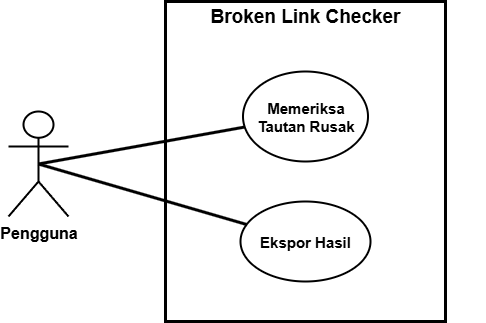
\includegraphics[width=0.5\textwidth]{Gambar/030301-use-case-diagram.png}
    \caption{Diagram \textit{use case} aplikasi}
    \label{fig:use-case-diagram}
\end{figure}

\subsection{Kebutuhan Fungsional}
\label{subsec:0303-kebutuhan-fungsional}

Kebutuhan fungsional berikut menggambarkan layanan inti yang harus disediakan oleh aplikasi desktop pemeriksa tautan rusak pada situs web:

\begin{enumerate}
    \item \textbf{Input URL}\\
    Sistem harus dapat menerima masukan berupa URL dari pengguna sebagai titik awal pemeriksaan.

    \item \textbf{Tampilan hasil secara \textit{streaming}}\\
    Sistem menampilkan daftar tautan yang ditemukan dari halaman web secara langsung (\textit{streaming}) selama proses pemeriksaan berlangsung.

    \item \textbf{Penghentian proses}\\
    Sistem menyediakan mekanisme bagi pengguna untuk menghentikan proses pemeriksaan kapan saja.

    \item \textbf{Mekanisme \textit{retry}}\\
    Sistem melakukan percobaan ulang terhadap tautan yang gagal diperiksa akibat kesalahan sementara, misalnya \textit{timeout} atau gangguan jaringan.

    \item \textbf{Ringkasan hasil}\\
    sistem menampilkan ringkasan berisi jumlah tautan yang diperiksa, jumlah tautan rusak, jumlah tautan yang terblokir, dan status proses pemeriksaan.


    \item \textbf{Sumber tautan rusak}\\
    Sistem menampilkan lokasi atau halaman tempat tautan rusak ditemukan, sehingga pengguna dapat menelusuri asal masalah.

    \item \textbf{Ekspor hasil}\\
    Sistem dapat mengekspor hasil pemeriksaan ke dalam berkas Excel agar mudah disimpan, dibagikan, atau dianalisis lebih lanjut.
\end{enumerate}





\subsection{Kebutuhan Non-Fungsional}
\label{subsec:0303-kebutuhan-non-fungsional}

Selain fungsi inti, sistem juga harus memenuhi sejumlah kebutuhan non-fungsional agar pemeriksaan tautan dapat berjalan stabil, efisien, dan mudah digunakan. Kebutuhan non-fungsional yang ditetapkan adalah sebagai berikut:

\begin{enumerate}
    \item \textbf{Antarmuka pengguna}\\
    Sistem disajikan dalam bentuk aplikasi desktop berbasis JavaFX dengan tampilan yang sederhana, tabel yang mudah dibaca, serta kontrol proses yang jelas.

    \item \textbf{Kinerja pemeriksaan}\\
    Sistem mampu menangani jumlah tautan yang besar dengan tetap menjaga waktu tanggap yang wajar. Hal ini dicapai dengan penerapan batas waktu (\textit{timeout}) pada setiap permintaan.

    \item \textbf{Pengendalian laju}\\
    Sistem membatasi jumlah permintaan dalam satuan waktu (\textit{rate limiting}) untuk mencegah server tujuan terbebani dan mengurangi risiko pemblokiran.

    \item \textbf{Eksekusi paralel}\\
    Sistem mendukung eksekusi permintaan secara paralel (\textit{concurrency}) khusus pada tahap pemeriksaan tautan agar proses lebih cepat. Jumlah permintaan simultan dibatasi agar tetap stabil dan tidak menimbulkan masalah \texttt{429 Too Many Requests} atau pemblokiran.

    \item \textbf{Ketahanan terhadap HTML tidak valid}\\
    Sistem mampu mengurai dokumen HTML yang tidak sesuai standar dengan bantuan Jsoup, sehingga tautan tetap dapat diekstrak meskipun struktur dokumen bermasalah.

    \item \textbf{Konsistensi identifikasi URL}\\
    Setiap URL dinormalisasi dan dicatat dalam repository untuk memastikan satu sumber daya hanya diperiksa sekali, sehingga hasil pemeriksaan konsisten dan tidak ada duplikasi.

    \item \textbf{Pelabelan hasil yang jelas}\\
    Setiap hasil pemeriksaan ditampilkan dengan kode status HTTP beserta keterangan resminya, serta pesan khusus untuk kesalahan non-HTTP seperti \textit{timeout}, \textit{bad host}, atau kesalahan koneksi.

    \item \textbf{Etika \textit{crawling}}\\
    Setiap permintaan menyertakan identitas \texttt{User-Agent}. Sistem juga menyediakan pengaturan jeda permintaan untuk menjaga agar aktivitas pemeriksaan tidak membebani server.

\end{enumerate}


